\documentclass{beamer}

\usepackage[ngerman]{babel}
\usepackage[utf8]{inputenc}

\usepackage{listings}
\setbeamercovered{transparent}

\usepackage[percent]{overpic}

\lstset{
  language=prolog,
  showstringspaces=false,
  aboveskip=-33pt
}

%\usetheme{Boadilla}
%\usetheme{Rochester}
%\usetheme{Rochester}
\usetheme[]{Goettingen}

%Kopf- und Fußzeile definieren
\setbeamertemplate{headline}
{%
\begin{overpic}[width=\paperwidth]
{kopf-hg.png}%
  \put(0,0){{~}{~}}%
\end{overpic}
}

\usecolortheme{dove} % :-)

\setbeamercovered{transparent}
\beamertemplatenavigationsymbolsempty
\setbeamertemplate{footline}[frame number]

%Titelseite
\title{Gestaltung von Prozessketten}
\author[A. Kazakova, B. Lüers]{Anastasia Kazakova, Bengt Lüers}

\institute[Universität Oldenburg]{
  \inst{}Fakultät 2 - Informatik, Wirtschafts- und Rechtswissenschaften}
  \titlegraphic{\includegraphics[scale=.4]{unisignet_r08_c2_cutted.png}
}

\date{\today}

\begin{document}

 \frame{\titlepage}

 \frame{\frametitle{Inhaltsverzeichnis}\tableofcontents[]}

 \section[Einleitung]{Einleitung}

 %schönes Zitat aus dem Buch
 \begin{frame}


 \textsc{\flqq If you can't describe what you are doing as a process, you don't know what you are doing.\frqq}
 \\
 \medskip
 \begin{flushright}
   \begin{small}
    \emph{\textit{W. Edwards Deming, \\
        Amerikanischer Unternehmensberater \\
        und Professor an der Columbia Universität}}
  \end{small}
 \end{flushright}

 \end{frame}

 \begin{frame}
  \frametitle{Prozess. Prozesstypen. Prozessstruktur}

  \textsc{Prozess} ist eine Folge von Aktivitäten zur Erstellung einer Leistung mit einem Anfang, einem Ende und einem Ziel.

\bigskip
  \textsc{Prozesstypen}\\
  \begin{itemize}
    \item Kernprozess
    \item Steuerungsprozess
    \item Unterstützungsprozesse
  \end{itemize}

\bigskip

\textsc{Prozessstruktur}

\end{frame}




 \section[Prozessketten]{Prozessketten}
 \begin{frame}
  \frametitle{Prozessstrukturanalyse}

  Prozessstrukturanalyse beschreibt, welche Aktivitäten in welcher Reihenfolge von wem durchgeführt werden. Durch diese Analyse können die Prozessabläufe gut visualisiert werden. \\
    \end{frame}

  \begin{frame}
    \frametitle{Grunde der Analyse}
   \begin{itemize}
      \item um herauszufinden, ob die Prozesse optimal gestaltet sind
      \item um die Redundanzen und Irrläufer in der Struktur zu erkennen
      \item um die Optimierungsansätze sinnvoll anwenden zu können
    \end{itemize}
  \end{frame}


 \begin{frame}
  \frametitle{Analysemethoden}

  \begin{itemize}
   \item Spaghetti-Diagramm
   \begin{itemize}
    \item graphische Darstellung auf hohem Aggregationsniveau
    \item identifiziert wesentliche Prozessschwachstellen
    \item eignet sich für deren Optimierung
   \end{itemize}
   \bigskip
    \item Ereignisorientierte Prozesskette
    \begin{itemize}
    \item stellt Details von Prozessen dar
    \item Erkennt Detailprobleme
    \item eignet sich fürs deren Beseitigen
   \end{itemize}

  \end{itemize}


 \end{frame}

 \subsection[Spaghettidiagramme]{Spagehttidiagramme}
 \begin{frame}
  \frametitle{Hintergründe}

 \end{frame}

 \subsubsection[Syntax]{Syntax}
 \begin{frame}
  \frametitle{Hintergründe}

 \end{frame}

 \subsection[Beispiel IBM]{Beispiel IBM}
 \begin{frame}
  \frametitle{IBM-Kreditvergabe: Ausgangssituation}
  Prozess
  \begin{itemize}
    \item Aufträge werden über Tocherunternehmen finanziert
    \item 5 Mitarbeiter eingebunden:
    \begin{itemize}
      \item 1 Telefonistin nimmt Antrag auf
      \item 3 Experten prüfen und definieren Kondititionen
      \item 1 Schreibkraft verfasst Angebot
    \end{itemize}
  \end{itemize}
  Auswirkungen
  \begin{itemize}
    \item Intransparenz
    \item 6 Tage Durchlaufzeit
    \item Kunden lassen Aufträge platzen
  \end{itemize}
 \end{frame}

 \begin{frame}
  \frametitle{IBM-Kreditvergabe: Prozessanalyse}
  Prozessanalyse
  \begin{itemize}
    \item Vorgang muss nur 90 Minuten dauern
    \item Übrige Zeit wird durch Warten und Informationsweitergabe verbraucht
  \end{itemize}
 \end{frame}

 \begin{frame}
  \frametitle{IBM-Kreditvergabe: Endsituation}
  Prozess
  \begin{itemize}
    \item 4 Mitarbeiter eingebunden:
    \begin{itemize}
      \item 1 Case Manager übernimmt gesamten Ablauf
      \item Case Manager wird von Computersystem und
      \item 3 Experten unterstützt
    \end{itemize}
  \end{itemize}

  Auswirkungen
  \begin{itemize}
    \item Durchgehender Ansprechpartner
    \item 4 Stunden Durchlaufzeit
    \item Mitarbeiterzahl reduziert
    \item Durchsatz gesteigert
  \end{itemize}
 \end{frame}

 \begin{frame}
  \frametitle{IBM-Kreditvergabe: Visualisierung}
  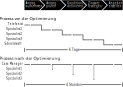
\includegraphics[scale=2.5]{4_5.png}
 \end{frame}

 \subsection{Optimierungsansätze}
 \begin{frame}
  \frametitle{Optimierungsansätze}
  Im Folgenden
  \begin{itemize}
    \item Zusammenfassungen bewährter Optimierungsansätze
  \end{itemize}
  Im Text
  \begin{itemize}
    \item Beispiele
  \end{itemize}
 \end{frame}

 \begin{frame}
  \frametitle{Entfallen}
   \begin{itemize}
    \item Ansatz: Aktivität lohnt sich nicht.
   \end{itemize}
  \centerline{\includegraphics[scale=2.5]{4_6_1.png}}
  \begin{itemize}
    \item Vorteil: Beschleunigung und Kostenersparnis.
    \item Nachteil: Geringer Nutzen entfällt.
  \end{itemize}
 \end{frame}

 \begin{frame}
  \frametitle{Beschleunigung}
  \begin{itemize}
    \item Ansatz: Standardisierung führt zu Zeiteffizienz.
  \end{itemize}
  \centerline{\includegraphics[scale=2.5]{4_6_2.png}}
  \begin{itemize}
    \item Vorteil: Sicherstellung einer Mindestqualität.
    \item Nachteil: Weniger Gestaltungspielraum.
  \end{itemize}
 \end{frame}

 \begin{frame}
  \frametitle{Zusammenlegung}
  \begin{itemize}
    \item Ansatz: Übergeben von Aufgaben dauert.
  \end{itemize}
  \centerline{\includegraphics[scale=2.5]{4_6_3.png}}
  \begin{itemize}
    \item Vorteil: Übertragungsfehler werden vermieden.
    \item Nachteil: Spezialisierungvorteile gehen verloren.
  \end{itemize}
 \end{frame}

 \begin{frame}
  \frametitle{Automatisierung}
  \begin{itemize}
    \item Ansatz: Routineaufgaben können automatisiert werden.
  \end{itemize}
  \centerline{\includegraphics[scale=2.5]{4_6_4.png}}
  \begin{itemize}
    \item Vorteil: Mittelfristige Einsparungen.
    \item Nachteil: Automatisierung erfordert hohe Investitionen.
  \end{itemize}
 \end{frame}

 \begin{frame}
  \frametitle{Verlagerung}
    \begin{itemize}
    \item Ansatz: Aktivitäten zwischen Akteuren verlagern.
  \end{itemize}
  \centerline{\includegraphics[scale=2.5]{4_6_5.png}}
  \begin{itemize}
    \item Vorteil: Akteure bekommen mehr Übersicht.
    \item Nachteil: Verlagerte Beanspruchung der Akteure.
  \end{itemize}
 \end{frame}

 \begin{frame}
  \frametitle{Reihenfolge}
    \begin{itemize}
    \item Ansatz: Sequenzen von Aktivitäten umstellen.
  \end{itemize}
  \centerline{
\includegraphics[scale=2.5]{4_6_6.png}}
  \begin{itemize}
    \item Vorteil: Erhöhte Flexibilität.
    \item Nachteil: Aufgabenübergabe braucht evtl. Zeit.
  \end{itemize}
 \end{frame}

 \begin{frame}
  \frametitle{Parallelisierung}
   \begin{itemize}
    \item Ansatz: Nebenläufigkeit von Aktivitäten ausnutzen.
   \end{itemize}
  \centerline{\includegraphics[scale=2.5]{4_6_7.png}}
  \begin{itemize}
    \item Vorteil: Massive Zeiteinsparungen möglich.
    \item Nachteil: Erhöhter Koordinationsaufwand.
  \end{itemize}
 \end{frame}

 \begin{frame}
  \frametitle{Vereinheitlichen der Verantwortung}
  \begin{itemize}
    \item Ansatz: \glqq One Face To The Customer\grqq
  \end{itemize}
  \centerline{\includegraphics[scale=2.5]{4_6_8.png}}
  \begin{itemize}
    \item Vorteil: Vermeiden von Übertragungsfehlern.
    \item Nachteil: Erhöhter Koodinationsaufwand.
  \end{itemize}
 \end{frame}

 \begin{frame}
  \frametitle{Arbeit in Interdisziplinären Teams}
  \begin{itemize}
    \item Ansatz: Experten-Gruppe kann mehr als ihre Mitglieder.
  \end{itemize}
  \centerline{
\includegraphics[scale=2.5]{4_6_9.png}}
  \begin{itemize}
    \item Vorteil: Effiziente Kommunikation.
    \item Nachteil: Klare Aufgabe und Anreize nötig.
  \end{itemize}
 \end{frame}

 \begin{frame}
  \frametitle{Leistungsmessung}
   \begin{itemize}
    \item Ansatz: Transparenz fördert Effizienz.
   \end{itemize}
  \centerline{
\includegraphics[scale=2.5]{4_6_10.png}}
  \begin{itemize}
    \item Vorteil: Mitarbeiter optimierien ihre Aufgaben selbst.
    \item Nachteil: Veröffentlichung muss durchgehalten werden.
  \end{itemize}
 \end{frame}

 \section[Ereignisorientierte Prozessketten]{Ereignisorientierte Prozessketten}
 \begin{frame}
  \frametitle{Hintergründe}

 \end{frame}

% Quellen

 \begin{frame}
  \frametitle{Quelle}
   \begin{itemize}
    \item Inhaltlich und alle Grafiken nach:\\
      Thonemann, Ulrich; Albers, Marco\\
      Operations Management:\\
      Konzepte, Methoden und Anwendungen\\
      Ulrich Thonemann. Unter Mitarb. von Marc Albers ... \\
      München [u.a.] : Pearson Studium, 2005. - 576 S.\\
      Ill., graph. Darst., Kt.\\
      Seite 153-163
   \end{itemize}
 \end{frame}

\end{document}
